\documentclass[linenumbers,trackchanges]{aastex7}
\begin{document}

\title{Larson Research Assignment Proposal}

\author[orcid=0000-0000-0000-0001,sname='Larson']{Colette Larson}
\affiliation{University of Arizona}
\email[show]{colettel1@arizona.edu}  

\section{Introduciton}
My proposed topic is to analyze how merging galaxies affect the structure of the remnant’s Halo. As galaxies merge, individual stars don't collide, but the original galaxies’ energies, gravitational forces and other orbital parameters interact with each other to create a remnant that is not simply the superposition of the colliding galaxies on top of each other, but rather a completely new structure \cite{10.1093/mnras/stz1306}. For my project I will take the simulation of the MW-M31 merge and analyze if the MW/M31 particles creates  structures within the remnants halo.

Understanding how galaxies merge is important because the universe is not static. It is constantly moving and expanding, resulting in galaxies running into each other and merging. Dark matter, in particular, is one of the driving forces of galaxy formation meaning "Dark matter haloes are the exclusive sites of galaxy, group, and cluster formation"\cite{10.1093/mnras/stz1306}. As such, studying the effects mergers have on halos  can give us valuable insight into not only on what will happen to merging galaxies but also valuable insight into how  galaxies are formed in the past. For example, we find that in simulated mergers “MHD halos are rounder than DMO halos at all radii” \cite{10.1093/mnras/stz2873}. It is often seen that older galaxies are smaller and less defined than new galaxies. Being able to analyze these galaxies would help us better understand whether this difference is due to mergers or some other factor of the early universe, like a change in angular momentum. 

One thing we know about galaxy mergers is that the shape of a remnant’s halo is greatly dependent on its energy and mass. If we define  the factors $\kappa $ and $\lambda$ such that:
\begin{eqnarray*}
\kappa \equiv \frac{E_0^{\prime }}{E_0} \left(\frac{M}{M^{\prime }} \right)^{5/3}, 
\lambda = \frac{\sqrt{|E_0|}|{\bf J}|}{GM^{5/2}} 
\end{eqnarray*}
We can see  a near perfect linear relationship with the ratio between the minor over the major axis (c/a) and minor over the intermediate axis (c/b) respectively, see figure 1 \cite{10.1093/mnras/stz1306}. We also know that the density profile of a halo is near universal "regardless of mass or cosmological model" \cite{10.1093/mnras/stz1307}. One of the most accurate version of these profiles is the Einasto profile, which is written as:
\begin{eqnarray*}
\rho (r) &=& \rho _{-2} \exp \left(-\frac{2}{\alpha _\mathrm{ E}}\left[\left(\frac{r}{r_{-2}}\right)^{\alpha _\mathrm{ E}} - 1 \right]\right) \, 
\end{eqnarray*}
in wich $\alpha _\mathrm{ E}$ is the Einasto shape parameter and ${r_{-2}}$ is the radius where the logarithmic slope is -2 \cite{10.1093/mnras/stz1307}. 
Another thing we know is the usual shape of halos. Studies have shown is that halos can be both triaxial and prolate (c/b $>$ b/a) with high mass haloes being less spherical then the less massive halo, and concentrated halos more spherical still \cite{10.1093/mnras/sty3531}.

\begin{figure}
    \centering
    \includegraphics[width=0.4\linewidth]{m_stz1306fig19.jpeg}
    \caption{oblateness of halo bases on $\kappa $ and  $\lambda $\cite{10.1093/mnras/stz1306}}
    \label{fig:enter-label}
\end{figure}

 One of the biggest questions in the realm of galaxy mergers is how do we simulate accurate mergers and the interactions between DM and baryons.We only recently learned that  these interactions like “stellar feedback and black hole feedback” are necessary to form disks and late time galaxies \cite{10.1093/mnras/stz2873}. Similarly N-body simulations do not perfectly model galaxy formation, because the interaction between baryons and DM “can have a significant impact on the structure of DM haloes especially in the inner halo where galaxies reside” \cite{10.1093/mnras/sty3531}. Another question is exactly what effect major mergers have on halo structure \cite{10.1093/mnras/stz1306}. While we have a general idea of what the result of a merge will look like and the main factors in said result, the fine details are still little understood. There is also the question of how we weigh what we know about gravitational potential from observational vs what we expect from the many galaxy formation models we have developed \cite{10.1093/mnras/stz2873}. The issue is made more complicated by our inability to properly model galaxy mergers.


\section{Proposal}
\subsection{This Proposal}

For my project I will determine how the shape remnant is effected by its component galaxies. Specifically, I will use the simulations of the MW and M31 merge which we have access and analyze how which parts of it are MW and which parts are M31. For example, do the MW and M31 particles stick together in the same groups or are they evenly distributed in the remnant? If the particles stick together, what do these structures look like? Are the structures spirals tor some form of triaxial ellipsoids? Does this shape vary by radius?

\subsection{Methods}

To determine the contribution of the MW vs. M31 halo particles to the final shape of the remnant. I will start by concatenating the snap 630 MW and M31 files. This snap is at time 9 gyr which is long enough after the merger the remnant should have settled. I will use the high-resolution files to avoid the 'noticeable differences' at low kpc from the center that some simulations experiences \cite{10.1093/mnras/stz2873}. Then I will use the code developed in Lab 7 to graph the density contour of the MW, M31, and the combined particles of the remnant. I will compare densities from both the front and sides of the galaxy (figure 2) as well as the radial density (figure 3).

\begin{figure}
    \centering
    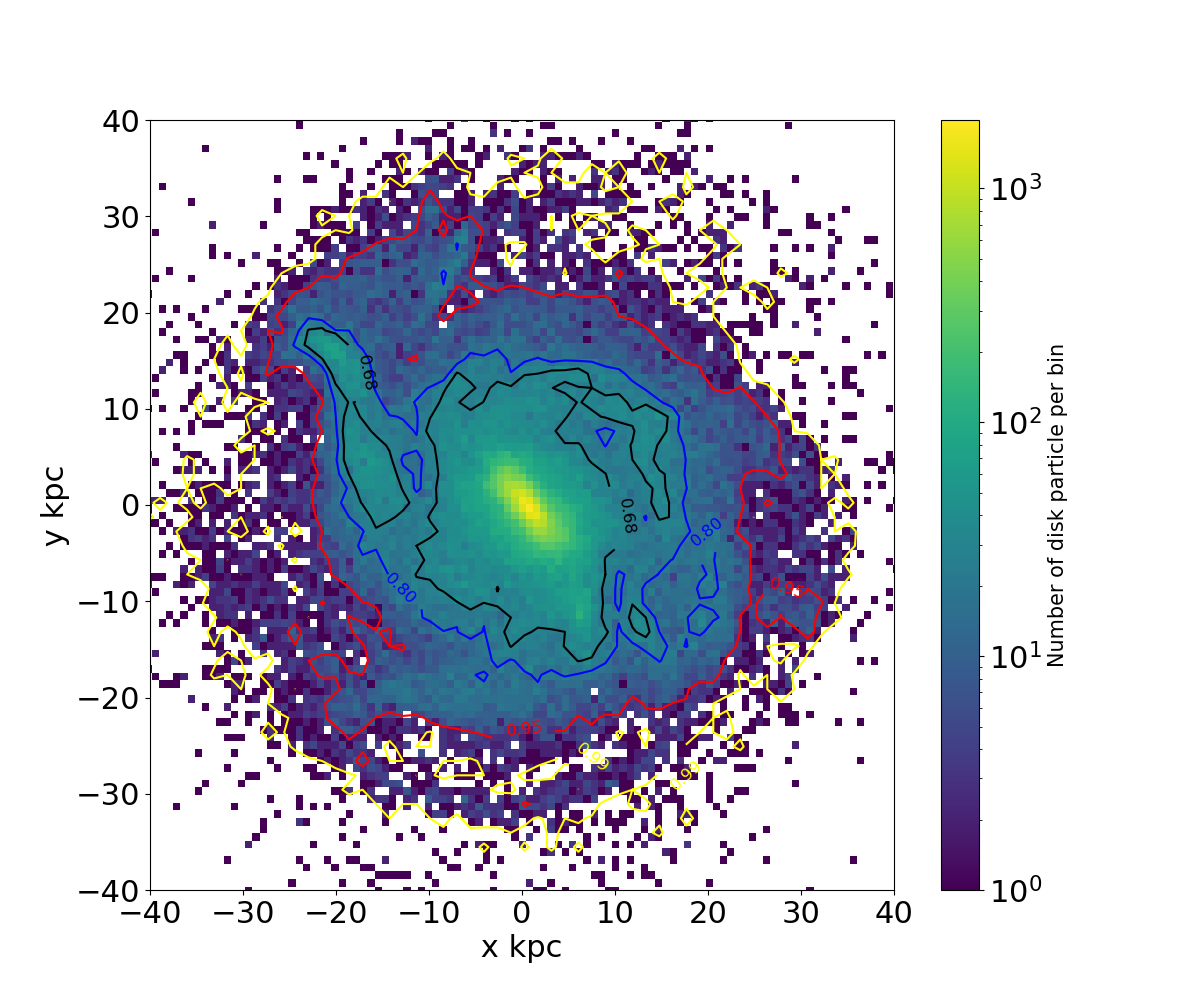
\includegraphics[width=0.5\linewidth]{Lab7_FaceOn_Density.png}
    \caption{Density Profile of M31 taken from a face on view taken from Lab 7. Density contorts are fit to the image}
    \label{fig:Lab7_FaceOn_Density}
\end{figure}

\begin{figure}
    \centering
    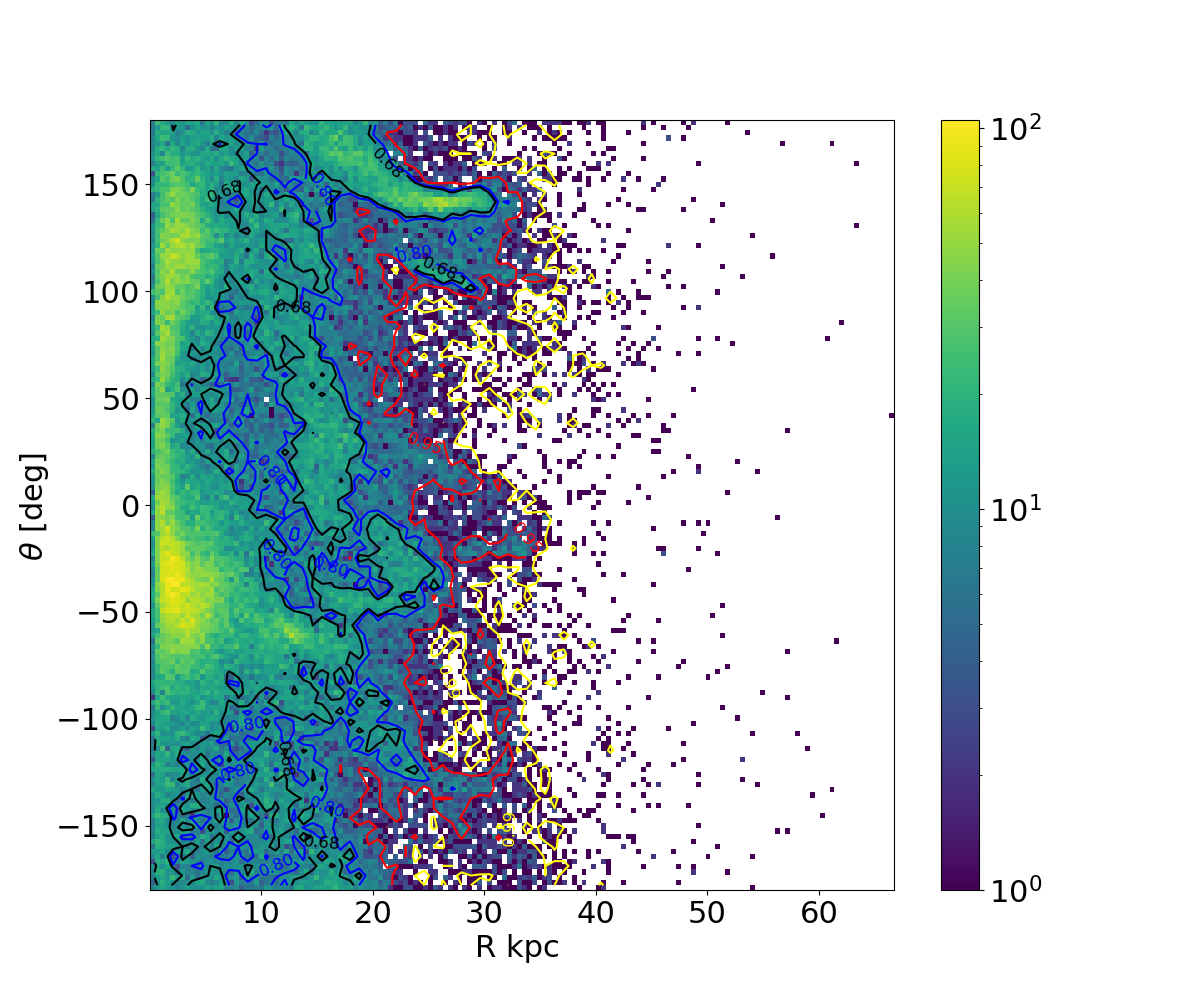
\includegraphics[width=0.5\linewidth]{Lab7_SpiralPhase.png}
    \caption{Density Profile of M31 as a function of Radius and angle taken from Lab 7. Density contorts are fit to the image}
    \label{fig:Lab7_SpiralPhase}
\end{figure}

\subsection{Hypothesis}

As MW and M31 are similar sizes/mass I expect for galaxies to mix nearly completely, resulting in a “near-complete mixing of old and new material” \cite{Frenk_2012}. Ergo I predict the remnant will be a triaxial ellipsoid with no significant structures. The core will likely be denser than the outer radii but there should not be any significant structures like arms or spirals.



\bibliography{References_Reasrch_Project_2}
\bibliographystyle{aasjournalv7}

\end{document}

